\section{The validity confirmation through the Union Bound}
\label{sec4}
%For a given RSC code, the distance spectrum provides information concerning the multiplicity of a codeword for a fixed weight and it is an effective tool to evaluate its error-correcting capability. In practice however, since higher-weight codewords have very little effect on its overall error-correcting capability, we usually use a partial distance spectrum, where the largest codeword weight value is set to $d_{\text{max}}$. 

%The distance spectrum of the RSC code can be obtained from its transfer function, denoted by $$T(Y,X)=\sum_{d=0}^{\infty}\sum_{w=0}^{\infty} a(d,w)Y^dX^w$$ where $a(d,w)$ is the number of codewords of weight $d$ generated by an input bit sequence of weight $w$. 
%The transfer function enumerates all the paths that diverge from and then return to the initial state \cite{ref3}, \textit{i.e.} the RTZ input paths. 
%Once the transfer function of an RSC code is known, it can be used to obtain bounds on the error-correcting capability using the union bound.
%Unfortunately, the complexity involved in deriving the transfer function increases as the number of states of the RSC code increases and other methods such as Mason's Rule \cite{ref3} have to be used. 

%For a given RSC code, we have shown in \ref{subsec:low-weight} that each codeword $c(x)$ is made up of $b(x)$ and $h(x)$ which have $a(x)$ as their common factor as shown in (\ref{novelEq2}) and (\ref{novelEq3}).
 In this section, In order to confirm the validity of our proposed method, we obtain a union bound using the list of low-weight codewords and compare it with that by transfer function and simulations.

To obtain a union bound, let $\cA_h(d)$ be the set of all $a(x)$ which yields weight-$d$ parity-check component \ie, $w_H(h(x))=w_H(a(x)f(x))=d$ for $a(x) \in \cA_h(d)$. 
Similarly, let $\cA_b(d)$ be the set of all $a(x)$ which yields weight-$d$ systematic component \ie, $w_H(b(x))=w_H(a(x)g(x))=d$, for $a(x) \in \cA_b(d)$
while the set of all $a(x)$ which yields weight-$d$ codeword \ie, $w_H(c(x))=w_H(a(x)f(x))+ w_H(a(x)g(x))=d$, is denoted by $\cA_c(d)$.

From \eqref{eq:cw-weight}, when $w_H(b(x)), w_H(h(x)) \geq 2$, we have
\begin{align}
\cA_c(d) = \bigcup_{\ell = 2}^{d-2} \left\{\cA_b(\ell) \cap \cA_h(d-\ell)\right\}
\label{Eq:exactset}
\end{align}
However, to determine $\cA_b(\ell)$ or $\cA_h(\ell)$ for a large $\ell$ is a complex task in general. Thus, in this paper, we replace the set $\cA_c(d)$ by the approximated set $\cA_c'(d)$, written as %\eqref{setApprox}
\begin{equation}
\begin{split}
\cA_c(d) \approx \cA_c'(d) &= \left\{\bigcup_{\ell = 2}^{\ell+1} \left\{\cA_b(\ell) \cap \cA_h(d-\ell)\right\}\right\}\bigcup \left\{\bigcup_{\ell = 2}^{\ell+1} \left\{\cA_b(d-\ell) \cap \cA_h(\ell)\right\}\right\}
\end{split}
\label{setApprox}
\end{equation}
where some codewords in $\cA_c(d)$ with $\ell \approx d-\ell$ may be ignored in $\cA_c'(d)$.
%We refer to the distance spectrum obtained using this method as the \textit{codeword component pattern distance spectrum}
%\begin{example}
%If we set $d=8$ and  $\alpha=1$, $\cA_c'(8)$ becomes
%\begin{equation*}
%\begin{split}
%\cA_c'(8) &=\left\{\left\{\cA_b(2) \cap \cA_h(6)\right\} \bigcup  \left\{\cA_b(3) \cap \cA_h(5)\right\} \right\} \bigcup \\
%& \left\{\left\{\cA_b(6) \cap \cA_h(2)\right\} \bigcup  \left\{\cA_b(5) \cap \cA_h(3)\right\} \right\} \\
%\end{split}
%\end{equation*}
%
%We can see that $\left\{\cA_b(4) \cap \cA_h(4)\right\}$ is not used in $\cA_c'(8)$, event though it is used in $\cA_c(8)$.
%\end{example}

%Once we obtain the set
% \begin{equation*}
% \bigcup_{d = d_{\text{min}}}^{d_{\text{max}}} \cA'_c(d) 
%\label{Eq:exactsetunion}
%\end{equation*}
%, we can list the low weight codeword component patterns for a given RSC code using \eqref{eq:low-weight-msg} and \eqref{eq:low-weight-parity}. 

% We set $d_{\text{max}}=d_{\text{min}}+3$ and  list the low weight codeword component patterns for the $5/7,~37/21$ and $23/35$ RSC codes in Tables \ref{novelTab13},  \ref{novelTab14} and \ref{novelTab15} respectively. 


%Having determined how to find valid values of $b(x)$ and $h(x)$ for Hamming weights $\leq 3$, we are now in a position to generate the codeword pattern distance spectrum for a given RSC code. We take a union bound like approach towards the generation of the codeword pattern distance spectrum. The approach is outlined below.
%\begin{enumerate}
 %\item Beginning with (\ref{novelEq2}), we find all values of $b(x),~w_H(b(x))=2$ that have the same roots as $g(x)$ and divide $g(x)$ by each valid polynomial to obtain the corresponding $a(x)$.\label{ubStep1}
 %\item Then using (\ref{novelEq3}), we multiply each $a(x)$ by $f(x)$ to obtain the corresponding value of $h(x)$. It is worth noting that $w_H(h(x))$ may be $\geq w_H(b(x))$. \label{ubStep2}
 %\item Since we are interested in only the low weight codewords, we ignore any $b(x) \st w_H(b(x))+w_H(h(x)) \geq d_{\text{max}}$. \label{ubStep3}
 %\item Next we set the weight value of $b(x)$ to $w_H(b(x))=3$, and repeat steps \ref{ubStep1} and \ref{ubStep2} while ignoring $b(x)$ that meet the condition in step \ref{ubStep3}.\label{ubStep4}
 %\item To obtain a complete codeword pattern distance spectrum, we do a reverse operation, \textit{i.e.} we focus on (\ref{novelEq2}) and find all values of $g(x),~w_H(\bh)=2$ that have the same roots as $f(x)$ and divide $f(x)$ by each valid polynomial to obtain the corresponding $a(x)$.
 %\item Then using (\ref{novelEq2}), we repeat steps \ref{ubStep2} through \ref{ubStep4}, being careful to avoid repitition.
 %\item Finally we arrange all valid values of $b(x)$ and $h(x)$ in ascending value of codeword weight,$w_H(b(x)) + w_H(h(x))$.
 %\end{enumerate}

%We use the codeword pattern distance spectrum to calculate the bit-error bounds for each RSC and compare them to the bit-error bounds obtained via the distance spectrum as well as simulation results. We use the probability of bit-error in doing this and a more general formula for calculating $P_b$ is shown below [4]:

%\begin{equation}
%P_b \leq \frac{1}{k} \sum_{d=d_{\text{free}}}^{\infty} w(d) Q\Bigg( \sqrt{\frac{2dE_c}{N_0}}\Bigg)
%\label{novelEq6}
%\end{equation}
%where $w(d)=\sum_{i=1}^{\infty} i~ a(d,i)$ and $ a(d,i)$ is the number of codewords of weight $d$ generated by an input message of weight $i$. If we set a limit on the maximum value of the codeword weight $d_{\text{max}}$
% we can rewrite (\ref{novelEq6}) as 
%\begin{equation}
%P_b \leq \frac{1}{k} \sum_{d=d_{\text{free}}}^{d_{\text{max}}} w(d) Q\Bigg( \sqrt{\frac{2dE_c}{N_0}}\Bigg)
%\label{novelEq7}
%\end{equation}
 %From the simulation results, we observed $d_{\text{max}}=d_{\text{min}}+3$ is a sufficient value for obtaining the BER bounds.
%In order to confirm the validity of our method, we use the values obtained from Tables \ref{novelTab8}, \ref{novelTab9} and \ref{novelTab10} to find the bounds for the BER of the RSC code, $P_b$.Finally, we compare the results obtained to $P_b$ found using the Transfer Function method as well as the simulation results.

%In order to validate our novel method, we can calculate the lower bound for each RSC code by modifying the union bound of the bit-error rate equation in \cite{ref4}, which gives us 
%\begin{align}
%P_b \leq \frac{1}{k} \sum_{d=d_{\text{free}}}^{\infty} \sum_{a(x) \in \cA_c(d)}w_H(a(x)g(x)) Q\Bigg( \sqrt{\frac{2dE_c}{N_0}}\Bigg)
%\label{novelEq6-1}
%\end{align}
%However, since the high-weight codewords have minor contribution on the unioin bound, \eqref{novelEq6-1} can be further approximated by setting a limit on the maximum value of the codeword weight $d_{\text{max}}$, resulting in
Finally, we obtain the following union bound as
\begin{align}
P_b \leq \frac{1}{k} \sum_{d=d_{\text{free}}}^{d_{\text{max}}} \sum_{a(x) \in \cA'_c(d)}w_H(a(x)g(x)) Q\Bigg( \sqrt{\frac{2dE_c}{N_0}}\Bigg)
\label{novelEq7}
\end{align}
where we let $d_{\text{max}}=d_{\text{free}}+3$. 

To verify the validity, assuming frame size $N=64$, we compared the bounds in \eqref{novelEq7} with that obtained using the transfer function method as well as the simulation results for the $5/7,~37/21$ and $23/35$ RSC codes.
%For each RSC code and a frame size of $N=64$, the codeword is BPSK modulated and transmitted over the AWGN channel. At the receiver end, the Viterbi algorithm is used to decode before a decision is made on the decoded sequence.

\begin{example}

%using our novel method outlined in the previous section,  we obtained the low-weight codeword component patterns for each RSC code and the results are shown in Tables \ref{novelTab13},  \ref{novelTab14} and \ref{novelTab15} respectively. We then calculate the lower bounds for our novel method and the transfer function using \eqref{novelEq7} and its original version in \cite{ref4} respectively. 
%It is worth noting that in all the tables, the codeword components are arranged in ascending order of codeword weight, with the $d_{\text{free}}$ components at the top of the table.  
%(quarantine)%For each RSC codeThese were obtained by dividing the general form of $h(x)$ for $w_H(\bh)=2$ and ($w_H(\bh)=2$ if it exists) by $f(x)$ and multiplying it by $g(x)$ to obtain $b(x)$ for a given RSC code. This process is repeated doing the same for the general form of $b(x)$. In both cases $a(x),~b(x)$ and $h(x)$ are only added to the list if $w_H(\bc) \leq d_{\text{max}}$.
The SC and PC components of 5/7 RSC are listed in Tables \ref{novelTab13}. For this code, since the feedforward connection has the polynomial representation $1+x^2$, the low-weight PCs are derived from Example \ref{ex-3}. On the other hand, for the feedback connection polynomial $1+x+x^2$, the details of low-weight patterns are demonstrated in Example \ref{ex-1}.

\begin{table}[htbp]
	\caption{SC and PC Components for the $5/7$ RSC code}
	\centering
	\begin{tabularx}{0.75\textwidth}{Xlll} 
		\hline
		$w_H(c(x))$& $a(x)$ & $b(x)$ & $h(x)$ \\ %[0.5ex] 
		\hline\hline
		5&$1$ & $1+x+x^{2}$ & $1+x^2$\\
		\hline\hline
		6&$1+x^2$ & $1+x+x^3+x^4$ & $1+x^{4}$\\
		%\hline
		&$1+x$ & $1+x^3$ & $1+x+x^2+x^3$\\
		\hline\hline
		&$1+x^2+x^4$ & $1+x+x^3+x^5+x^6$ & $1+x^{6}$\\
		%\hline\hline
		7&$1+x^2+x^3$ & $1+x+x^5$ & $1+x^3+x^4+x^5$\\
		%\hline
		&$1+x+x^2$ & $1+x^2+x^4$ & $1+x+x^3+x^4$\\
		%\hline
		&$1+x+x^3$ & $1+x^4+x^5$ & $1+x+x^2+x^5$\\
		\hline \hline
		8&$1+x^2+x^4+x^6$ & $1+x+x^3+x^5+x^7+x^8$ & $1+x^8$\\
		%\hline
		&$1+x+x^3+x^4$ & $1+x^6$ & $1+x+x^2+x^4+x^5+x^6$\\
		\hline
		%======extra
		%\hline
		%$1+x+x^3+x^5$ & $1+x^4+x^6+x^7$ & $1+x+x^2+x^7$\\
		%\hline
		%$1+x+x^2+x^4$ & $1+x^2+x^5+x^6$ & $1+x+x^3+x^6$\\
		%\hline
		%$1+x+x^2+x^3$ & $1+x^2+x^3+x^5$ & $1+x+x^4+x^5$\\
		%\hline
		%$1+x^2+x^3+x^5$ & $1+x+x^6+x^7$ & $1+x^3+x^4+x^7$\\
		%\hline
		%$1+x^2+x^3+x^4$ & $1+x+x^4+x^6$ & $1+x^3+x^5+x^6$\\
		%\hline
		%$1+x^2+x^4+x^5$ & $1+x+x^3+x^7$ & $1+x^5+x^6+x^7$\\
	\end{tabularx}
	
	\label{novelTab13}
\end{table}

\begin{figure}[htbp]
	\centering
	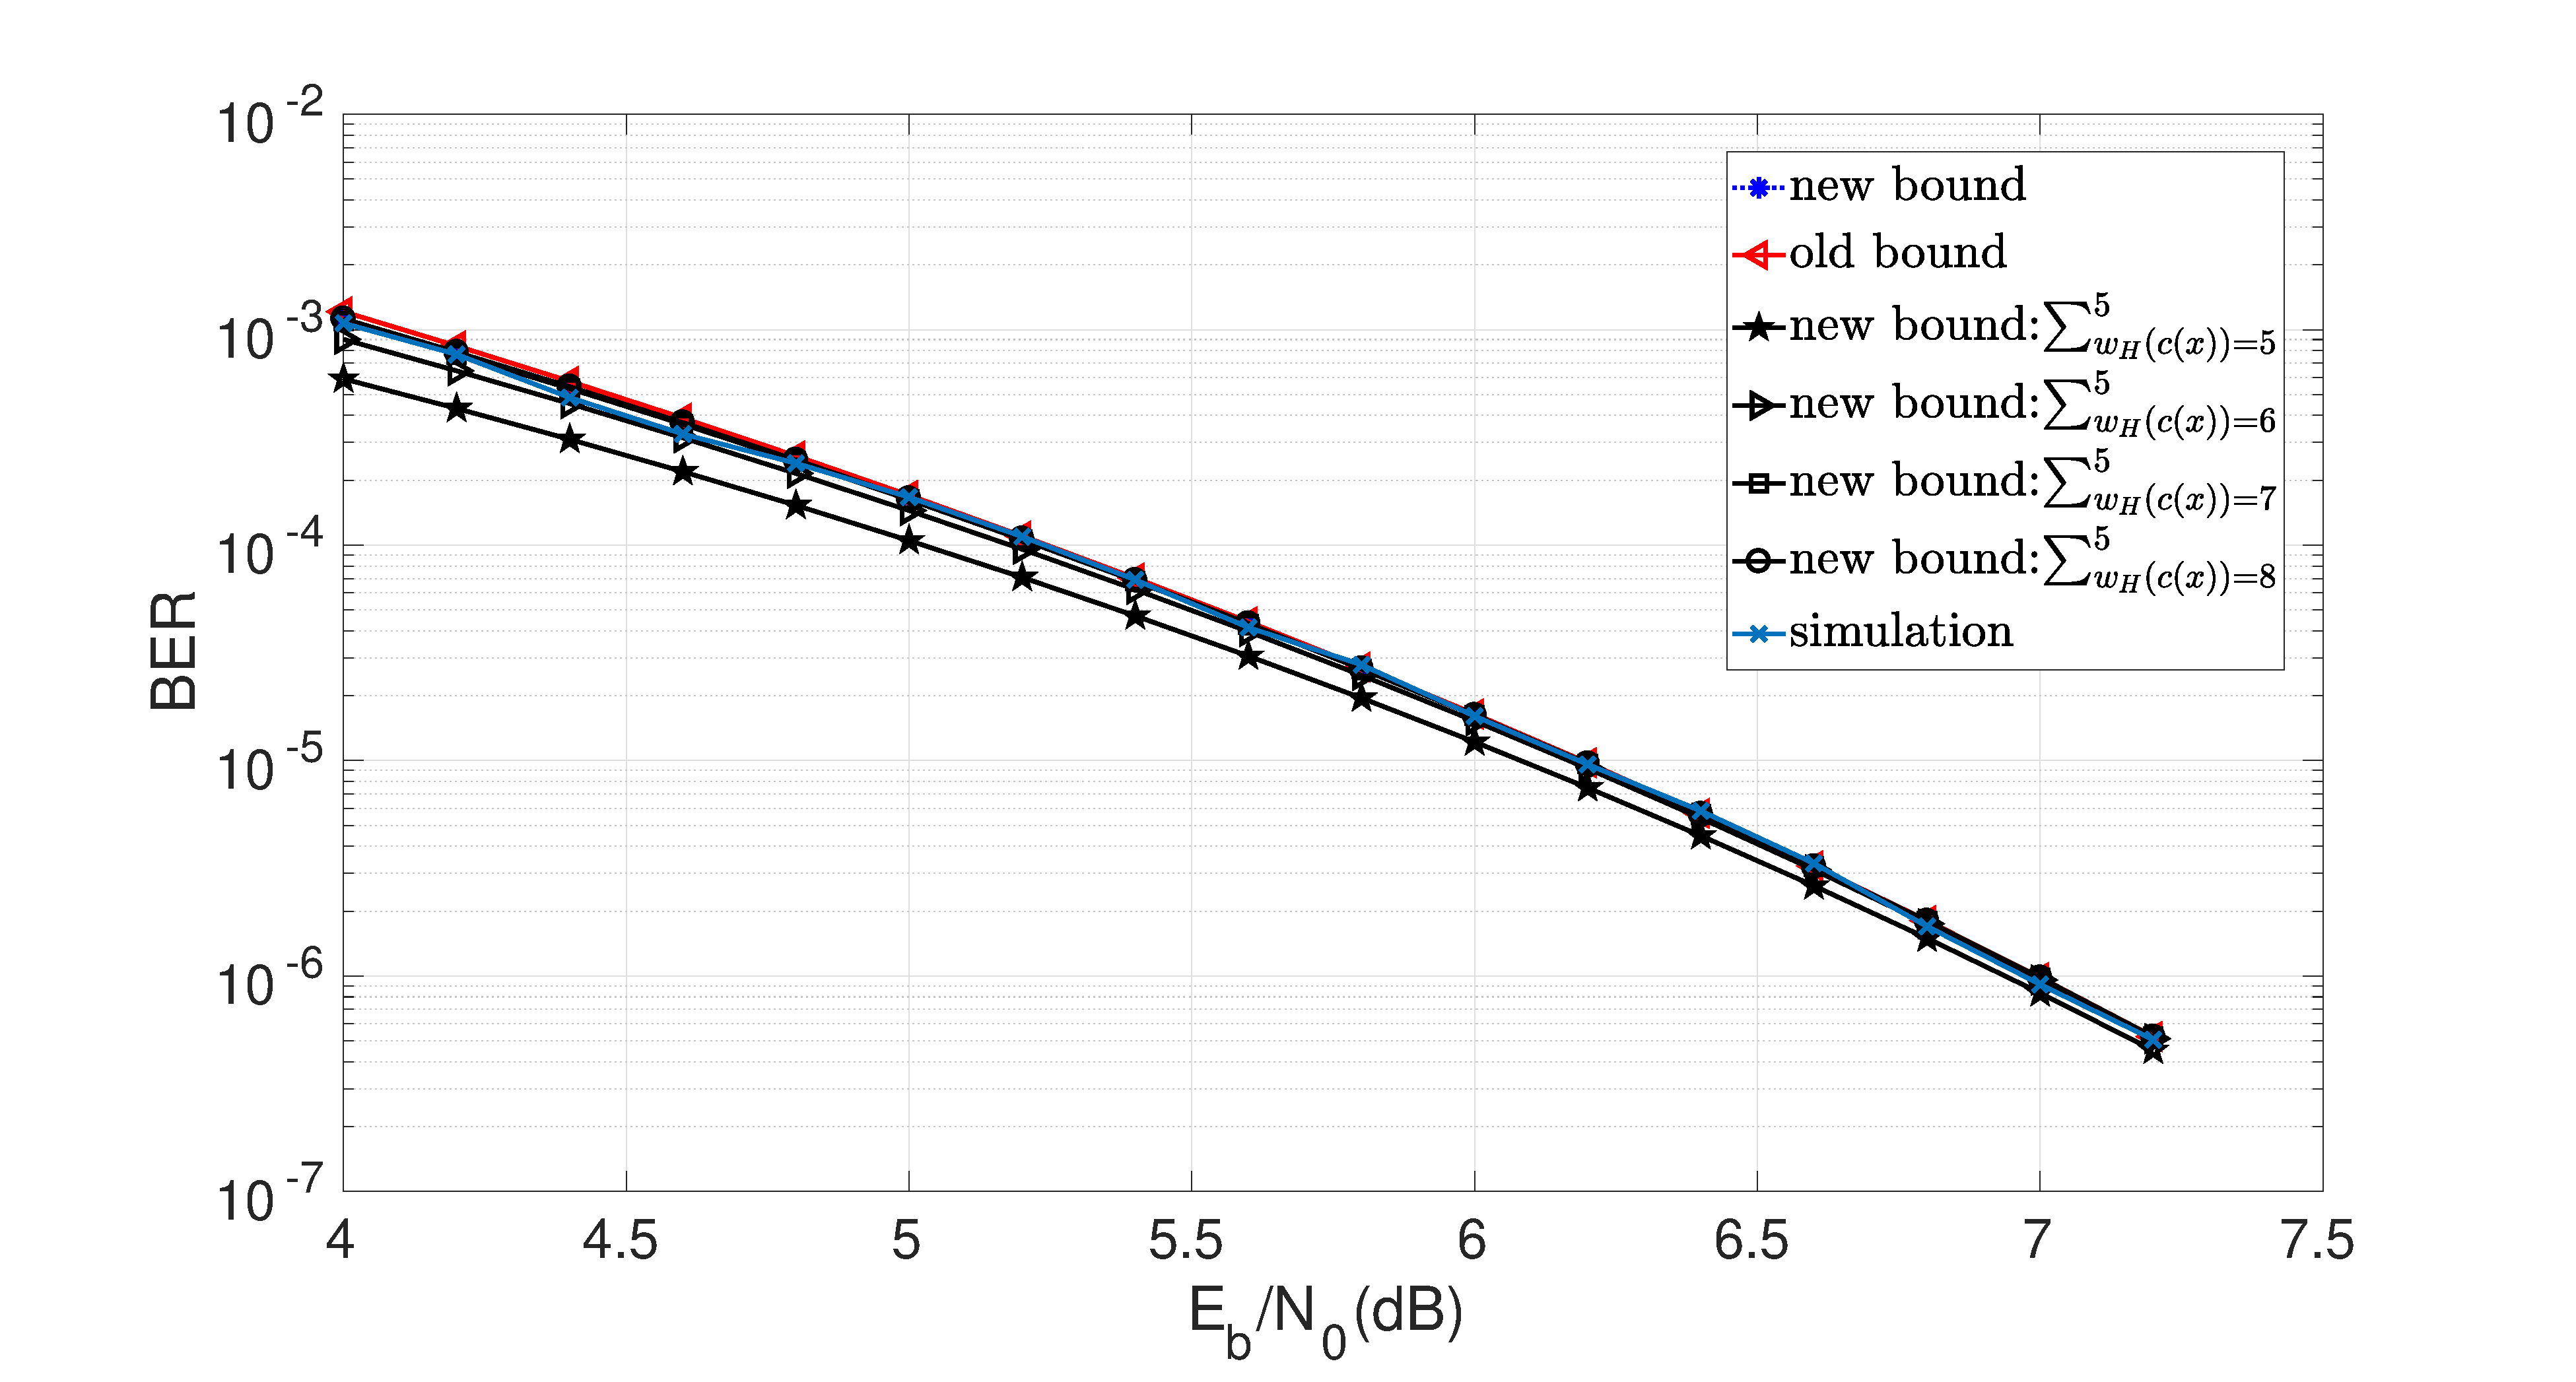
\includegraphics[width=0.5\textwidth]{./Images/RSC_5_7_lower_weights2.eps}
	\captionof{figure}{Old Bound vs New Bound vs Simulation for 5/7 RSC Code}
	\label{simFig1}
\end{figure}

Fig. \ref{simFig1} shows the simulation results for the $5/7$ RSC code as well as the lower bounds obtained using the transfer function as well as our novel method. We can observe that the accuracy of new (novel method) bound increases with the number of terms used in the approximation. Also, we can observe from this figure that there is some difference between the new (novel method) bound and the old (transfer function) bound, but they tend to converge as $E_b/N_0$ increases. This suggests that the approximation \eqref{setApprox} used in our novel method is sufficient for the $5/7$ RSC code.
\label{5/7graph}
\end{example}
%We observe that for both Fig. \ref{simFig1} and Fig. \ref{simFig2}, there is some difference between the new (novel method) bound and the old (transfer function) bound, but they tend to converge as $E_b/N_0$ increases. This suggests that the approximation used with our novel method is sufficient for these RSC codes.

%codewords generated considering $b(x),~w_H(b(x))>3$ as well as codewords which have a parity-check sequence $h(x),~w_H(h(x))>3$ do not have much effect on the BER of the code as $E_b/N_0$ increases.

%The gap that is observed in the low $E_b/N_0$ regions is attributed to omitting codewords generated by the RTZ inputs of weight $w_H(\bb)=4$ as well as codewords with parity-check sequences $w_H(\bh)=4$ in our calculation of the new bound. 

%Fig. \ref{simFig4} and Fig. \ref{simFig5} are similar to  Fig. \ref{simFig1} and Fig. \ref{simFig2}, with the only difference being that codewords generated by the RTZ inputs of weight $w_H(\bb)=4$ as well as codewords with parity-check sequences $w_H(\bh)=4$ have been added in our calculation of the new bound. The new and old bounds match up and the accuracy of our bound is greatly improved.The simulation results also agree with the bounds as they also converge with the bounds.

\begin{example}
For 37/21 RSC code, since the polynomials of feedforward and feedback connections are $1+x+x^2+x^3+x^4$ and $1+x^4$, respectively. Thus, the CS and PC components listed in Table \ref{novelTab14} can be obtained by the method demonstrated in Examples \ref{ex-2} and \ref{ex-3}, respectively.
\begin{table}[htbp]
	\caption{SC and PC Components for the $37/21$ RSC code, $d_{\text{free}}=6$}
	\centering
	\begin{tabularx}{0.75\textwidth}{Xlll} 
		\hline
		$w_H(c(x))$&$a(x)$ & $b(x)$ & $h(x)$ \\ [0.5ex] 
		\hline\hline
		6&$1+x$ & $1+x+x^{4}+x^5$ & $1+x^5$\\
		\hline\hline
		7&$1$ & $1+x^4$ & $1+x+x^2+x^3+x^4$\\
		\hline\hline
		8&$1+x+x^5+x^6$ & $1+x+x^4+x^6+x^9+x^{10}$ & $1+x^{10}$\\
		\hline
		%$1+x+x^4+x^5$ & $1+x+x^8+x^9$ & $1+x^4+x^5+x^9$\\
		%\hline
		%$1+x^2$ & $1+x^2+x^4+x^6$ & $1+x+x^5+x^6$\\
		%\hline
		%$1+x+x^5$ & $1+x+x^4+x^9$ & $1+x^6+x^7+x^8+x^9$\\
		%\hline
		%$1+x+x^4$ & $1+x+x^5+x^8$ & $1+x^4+x^6+x^7+x^8$\\
		%\hline
		%$1+x^2+x^4$ & $1+x^2+x^6+x^8$ & $1+x+x^4+x^7+x^8$\\
		%\hline
		%$1+x^3+x^4$& $1+x^3+x^7+x^8$ & $1+x+x^2+x^4+x^8$\\
		%\hline
		%$1+x^4+x^5$ & $1+x^5+x^8+x^9$ & $1+x+x^2+x^3+x^9$\\
	\end{tabularx}
	
	\label{novelTab14}
\end{table}

\begin{figure}[htbp]
	\centering
	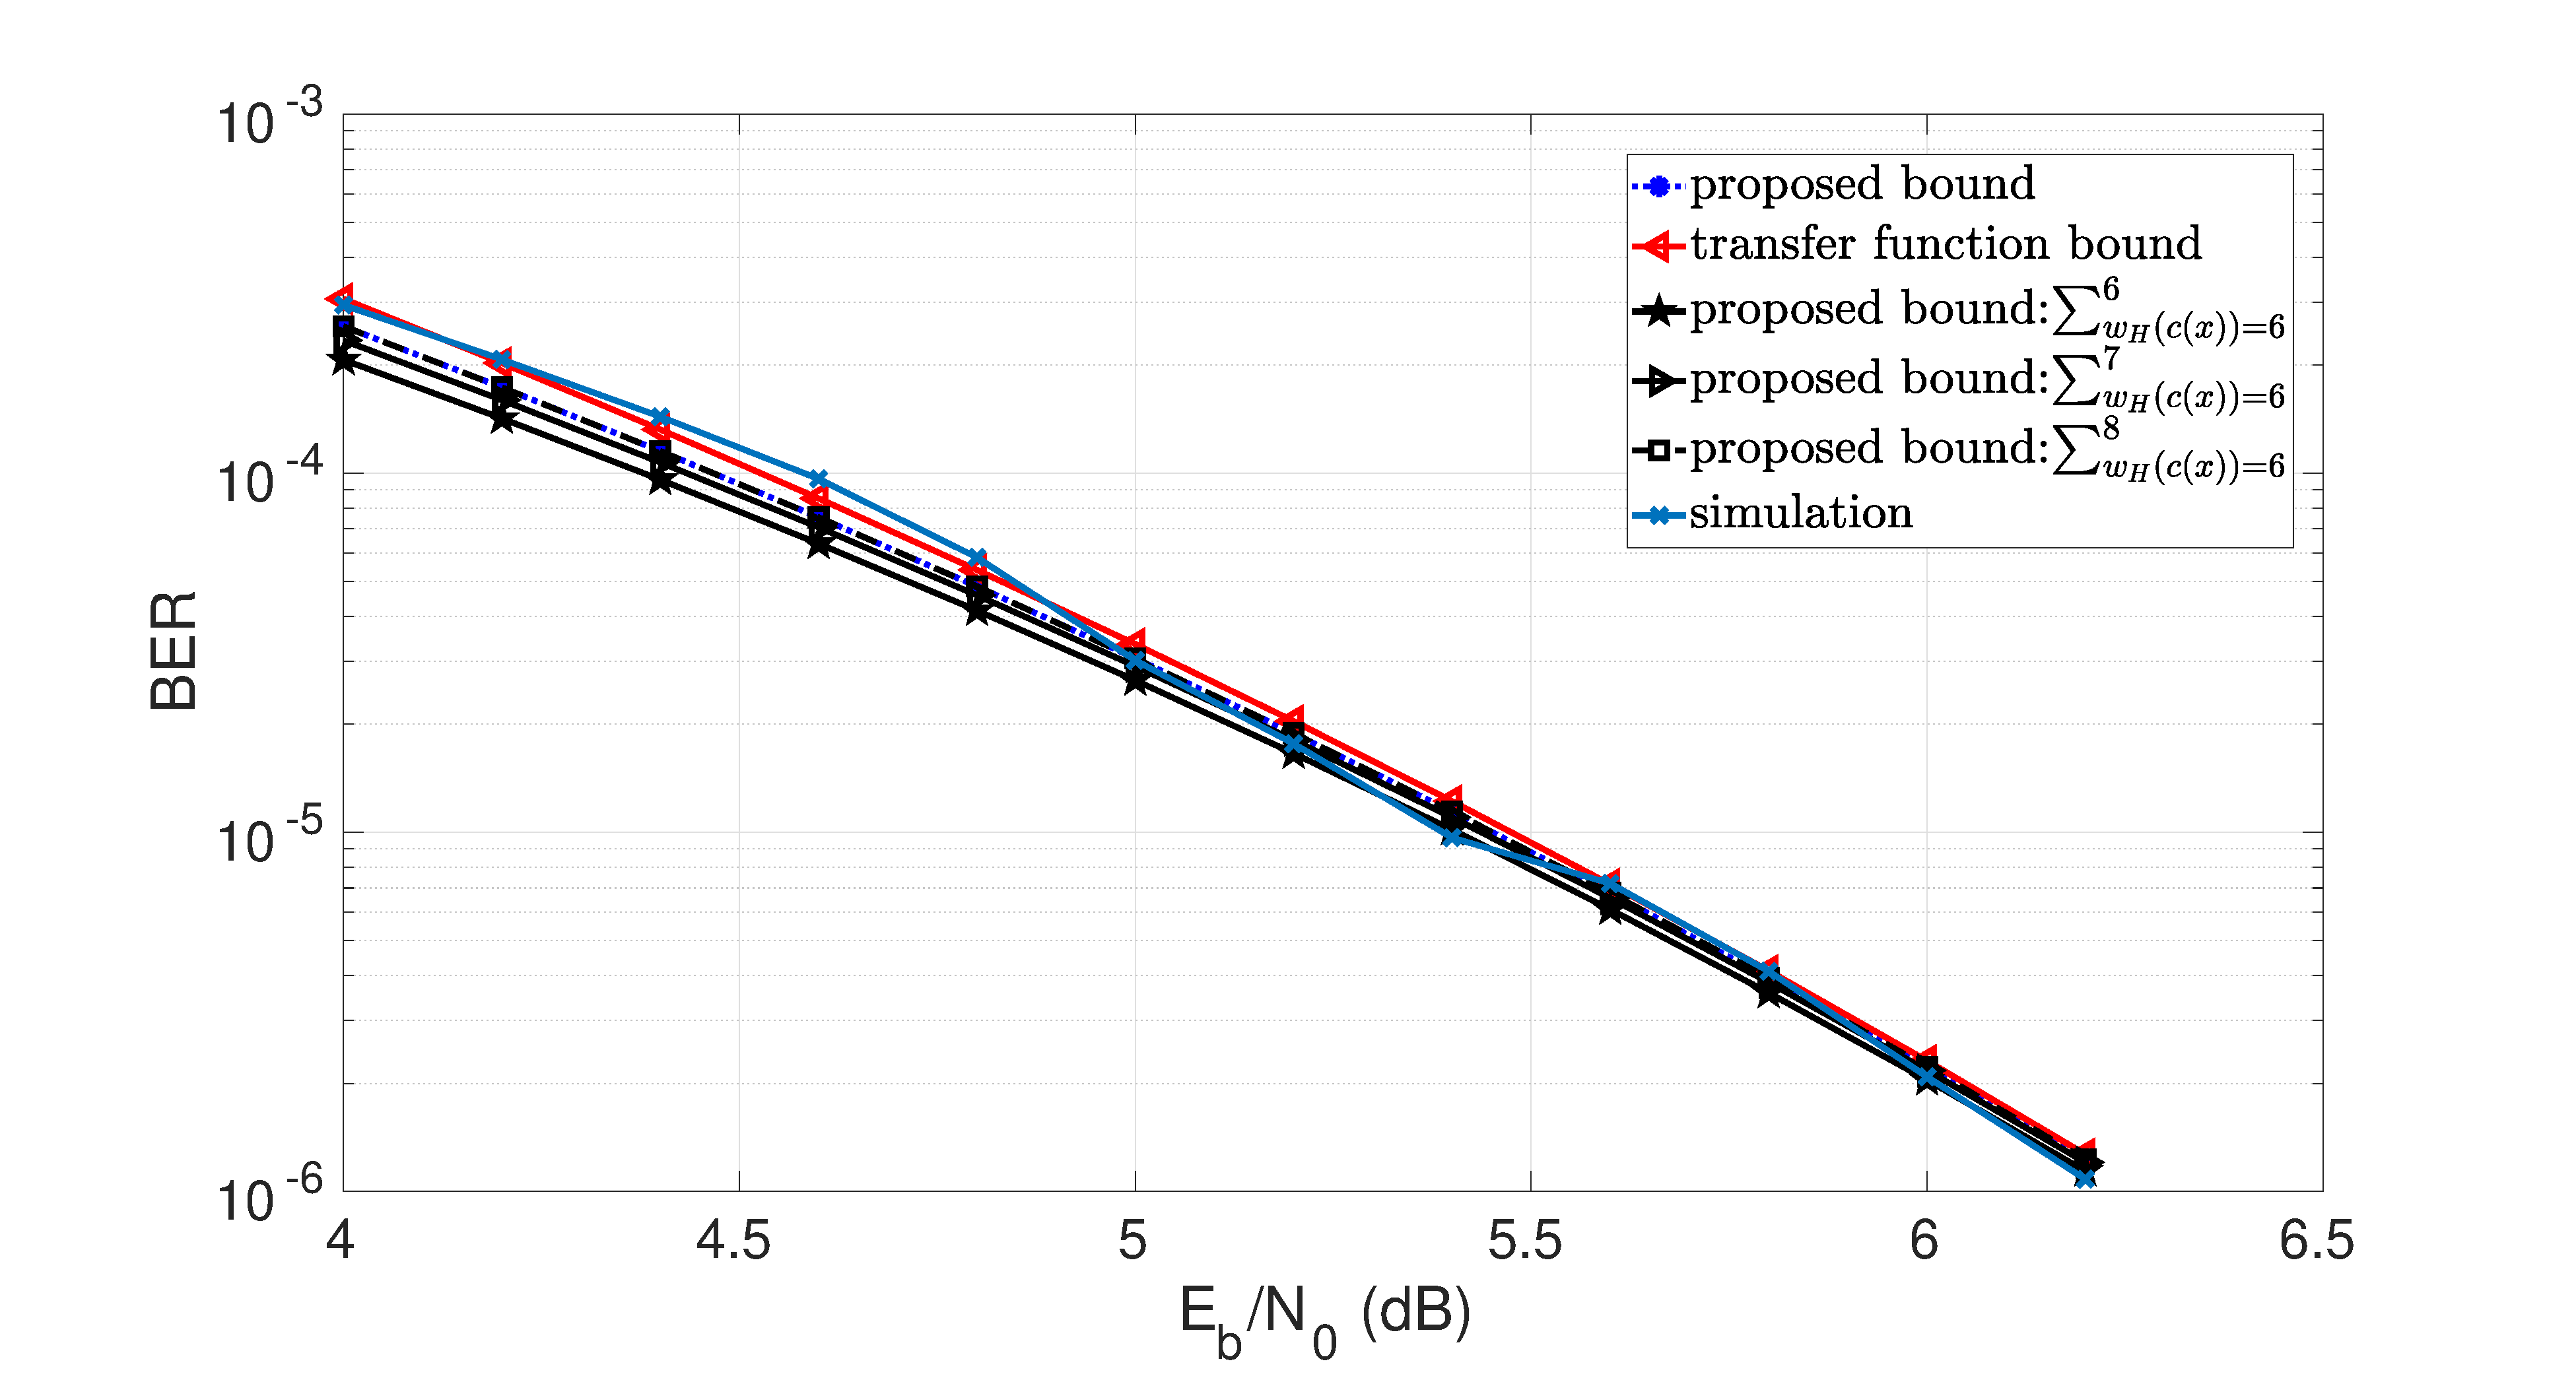
\includegraphics[width=0.5\textwidth]{./Images/RSC_37_21_lower_weights2.eps}
	\caption{Old Bound vs New Bound vs Simulation for 37/21 RSC Code}
	\label{simFig2}
\end{figure}
Fig. \ref{simFig2} shows the simulation results for the $37/21$ RSC code as well as the lower bounds obtained using the transfer function as well as our novel method. The bounds as well as the simulation results for this RSC code are shown in Fig. \ref{simFig2} and by observation, we can draw conclusions similar to  Example \ref{5/7graph} with respect to the accuracy of the novel method .

%, we observe that there is some difference between the new (novel method) bound and the old (transfer function) bound, but they tend to converge as $E_b/N_0$ increases. This suggests that the approximation $ \bigcup_{d = d_{\text{min}}}^{d_{\text{max}}} \cA'_c(d) $ used in our novel method is also sufficient for the $37/21$ RSC code.
%In \ref{simFig3}, we observe that the old bounds and simulation results converge as the Eb/No value increases. However, there is a very distinct gap between the new bound and the old bound. Moreover, the bounds do not converge as the Eb/No increases. This suggests that the approximation used in our novel method is insufficient for this RSC code and considering  $w_H(h(x)),~w_H(b(x))=4$ might yield a more accurate bound.
\end{example}

\begin{example}
\begin{table}[htbp]
	\caption{Partial Codeword Component Pattern Distance Spectrum for the $23/35$ RSC code, $d_{\text{free}}=7$}
	\centering
	\begin{tabularx}{0.75\textwidth}{lXlX} 
		\hline
		$w_H(c(x))$ & $a(x)$ & $b(x)$ & $h(x)$ \\ [0.5ex] 
		\hline\hline
		7&$1+x^2+x^3$ & $1+x^7$ & $1+x+x^2+x^6+x^7$\\
		\hline
		&$1$ & $1+x^2+x^3+x^4$ & $1+x+x^{4}$\\
		\hline \hline
		9&$1+x+x^2+x^3+x^5$ & $1+x+x^3+x^4+x^8+x^9$ & $1+x^7+x^9$\\
		\hline
		&$1+x+x^2+x^3+x^5+x^7+x^8$ & $1+x+x^3+x^4+x^7+x^{12}$ & $1+x^{11}+x^{12}$\\
		\hline\hline
		10&$1+x^2+x^3+x^7+x^9+x^{10}$ & $1+x^{14}$ & $1+x+x^2+x^6+x^8+x^9+x^{13}+x^{14}$\\
		\hline
	\end{tabularx}
	
	\label{novelTab15}
\end{table}

\begin{figure}[htbp]
	\centering
	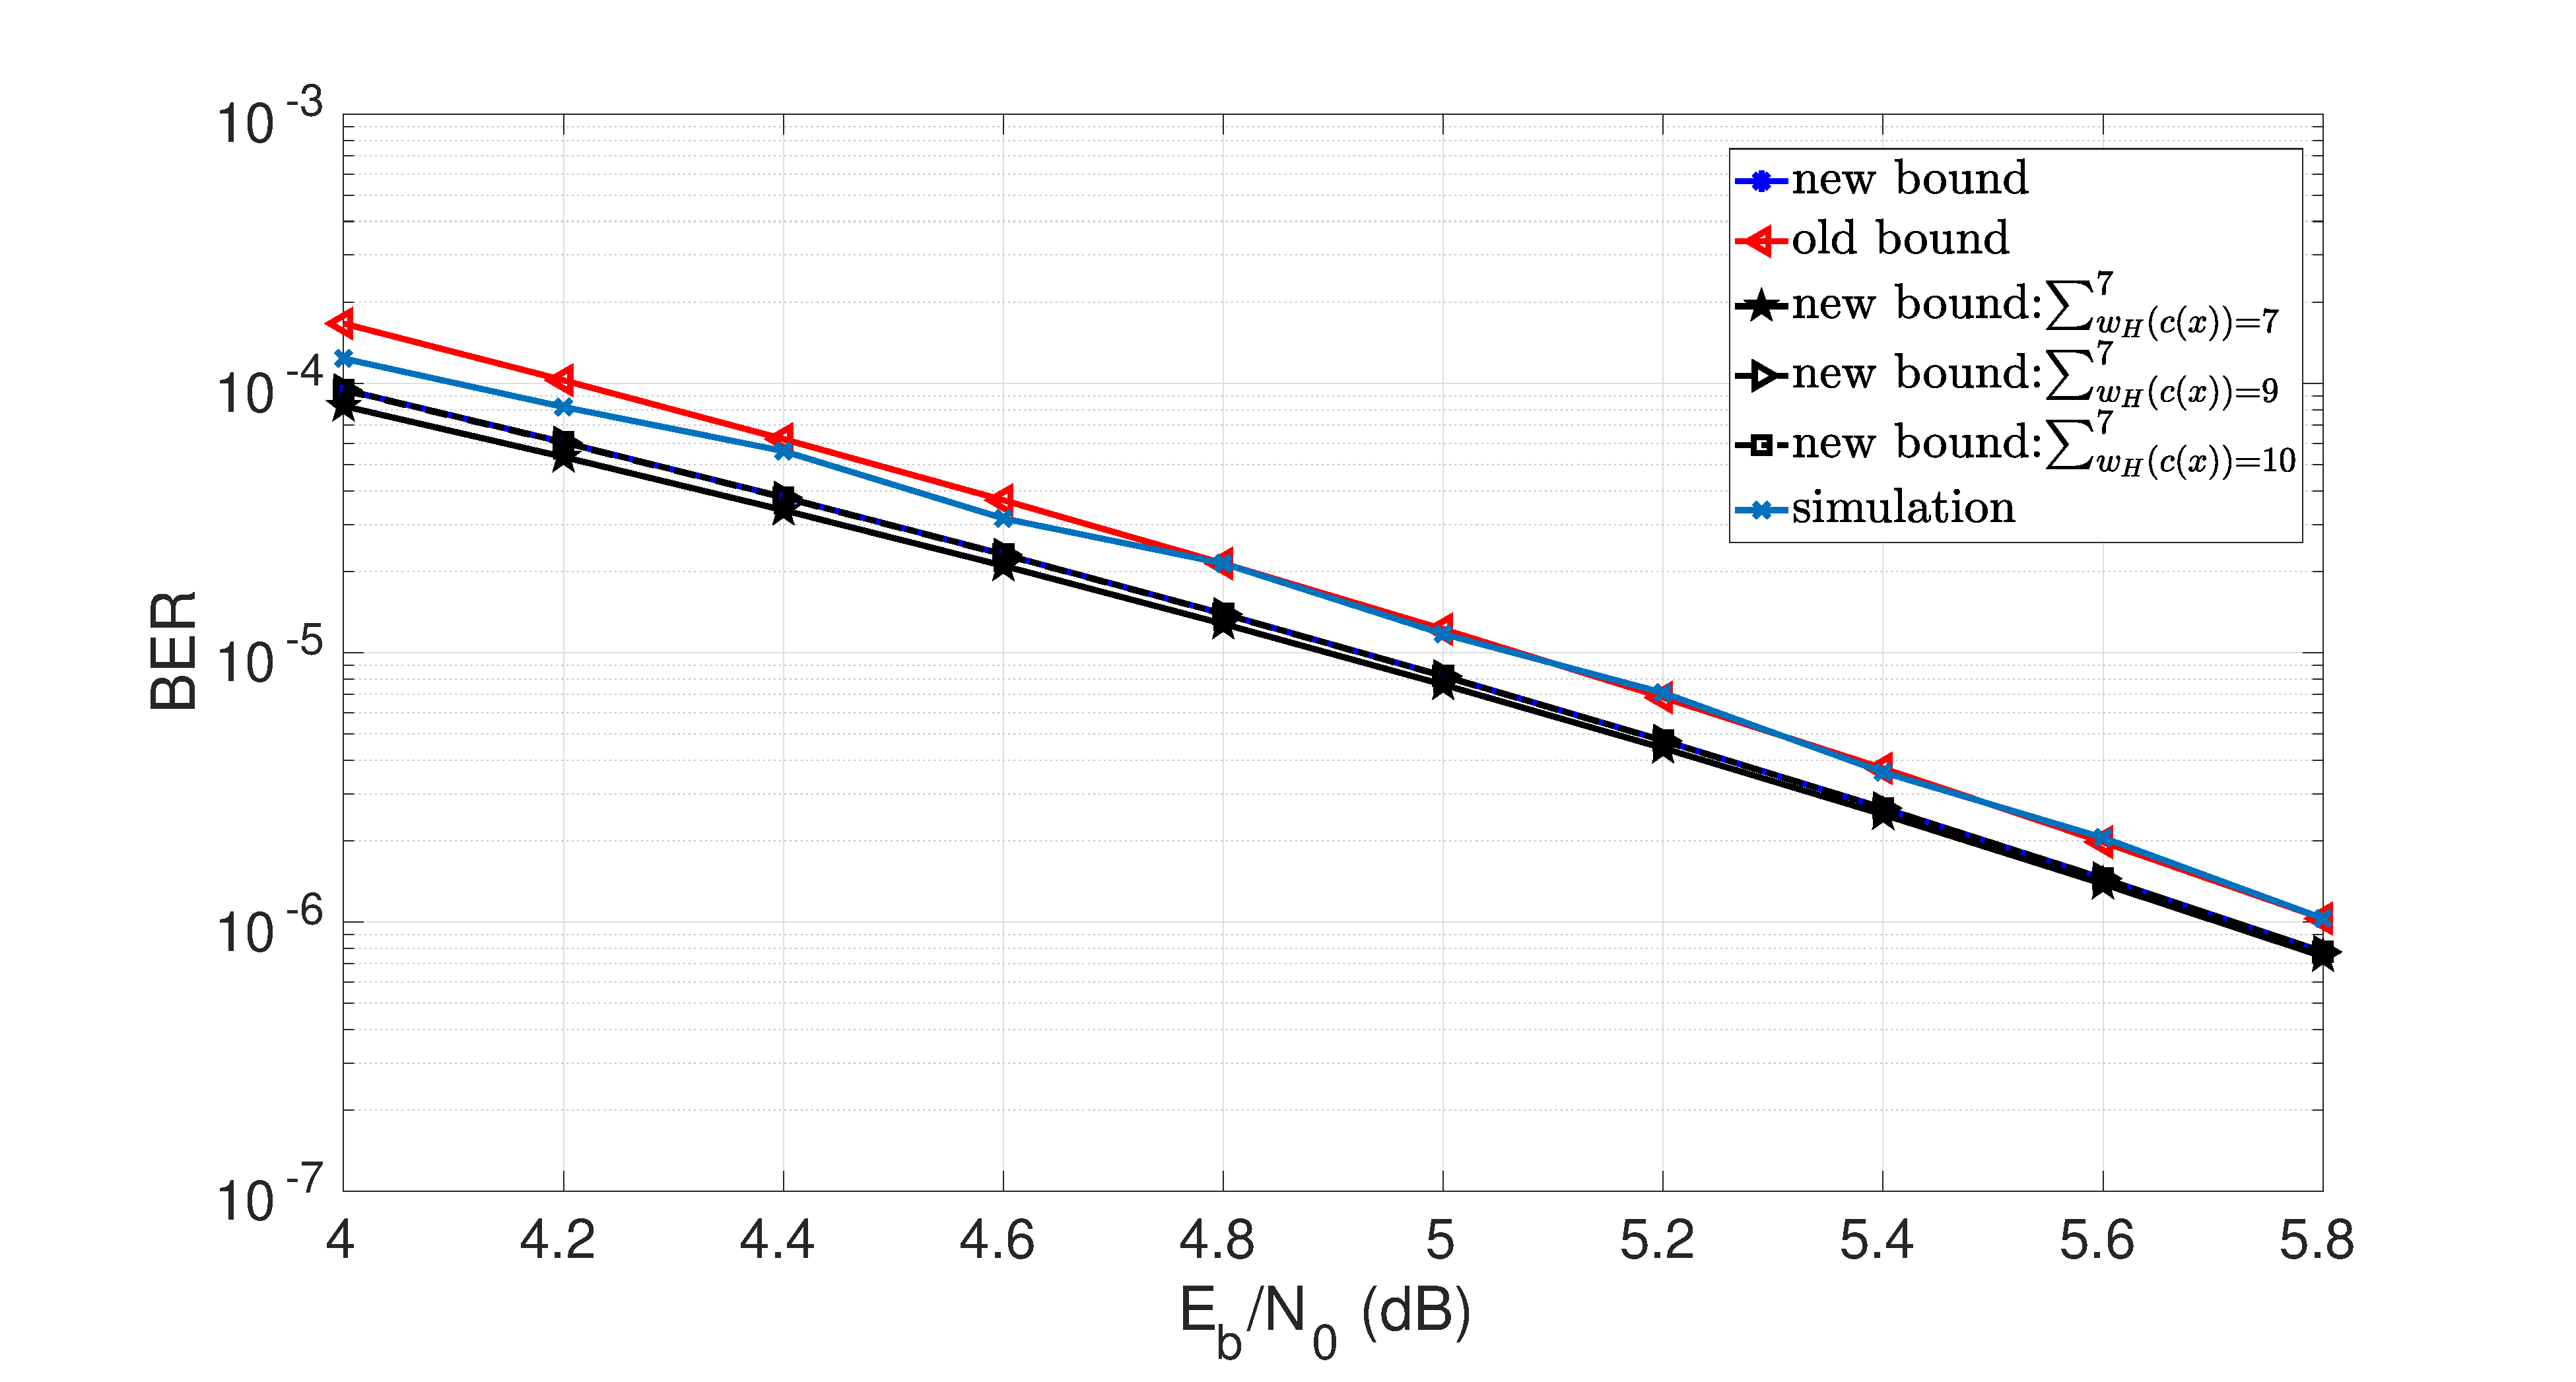
\includegraphics[width=0.5\textwidth]{./Images/RSC_23_35_lower_weights2.eps}
	\caption{Old Bound vs New Bound vs Simulation for 23/35 RSC Code}
	\label{simFig3}
\end{figure}
Fig. \ref{simFig3} shows the simulation results for the $23/35$ RSC code as well as the lower bounds obtained using the transfer function as well as our novel method. The feedforward connection has the polynomial representation $1+x+x^4$, which is similar in characteristic to the polynomial in Example \ref{ex-1}. It can easily be confirmed that there exists weight-2 and weight-3 PCs. For the weight-2 PCs, the general form for $a(x)$ is
\begin{equation*}
	a(x)=\sum_{\ell=0}^{L-1} x^{15\ell}(1+x+x^{2}+x^3+x^5+x^7+x^8+x^{11})
\end{equation*}
and since it yields codewords such that $w_H(c(x))>d_{\text{max}}$, there are not included in our approximation of the lower bound, as can be observed from Table \ref{novelTab14}. The feedback connection has the polynomial representation $1+x^2+x^3+x^4$, which can be factorized into $2$ irreducible polynomials and it can easily be confirmed that there exists no weight-3 SCs, since $1+x$ is a factor. In Fig. \ref{simFig3}, we observe that the old (transfer function) bounds and simulation results converge as the $E_b/N_0$ value increases. However, there is some difference between the new (novel method) bound and the old (transfer function) bound, even as $E_b/N_0$ increases. This suggests that the approximation used in our novel method is insufficient for this $23/35$ RSC code and considering  $w_H(h(x)),~w_H(b(x))=4$ might yield a more accurate bound.
\end{example}

%\begin{figure}[h!]
%\centering
%		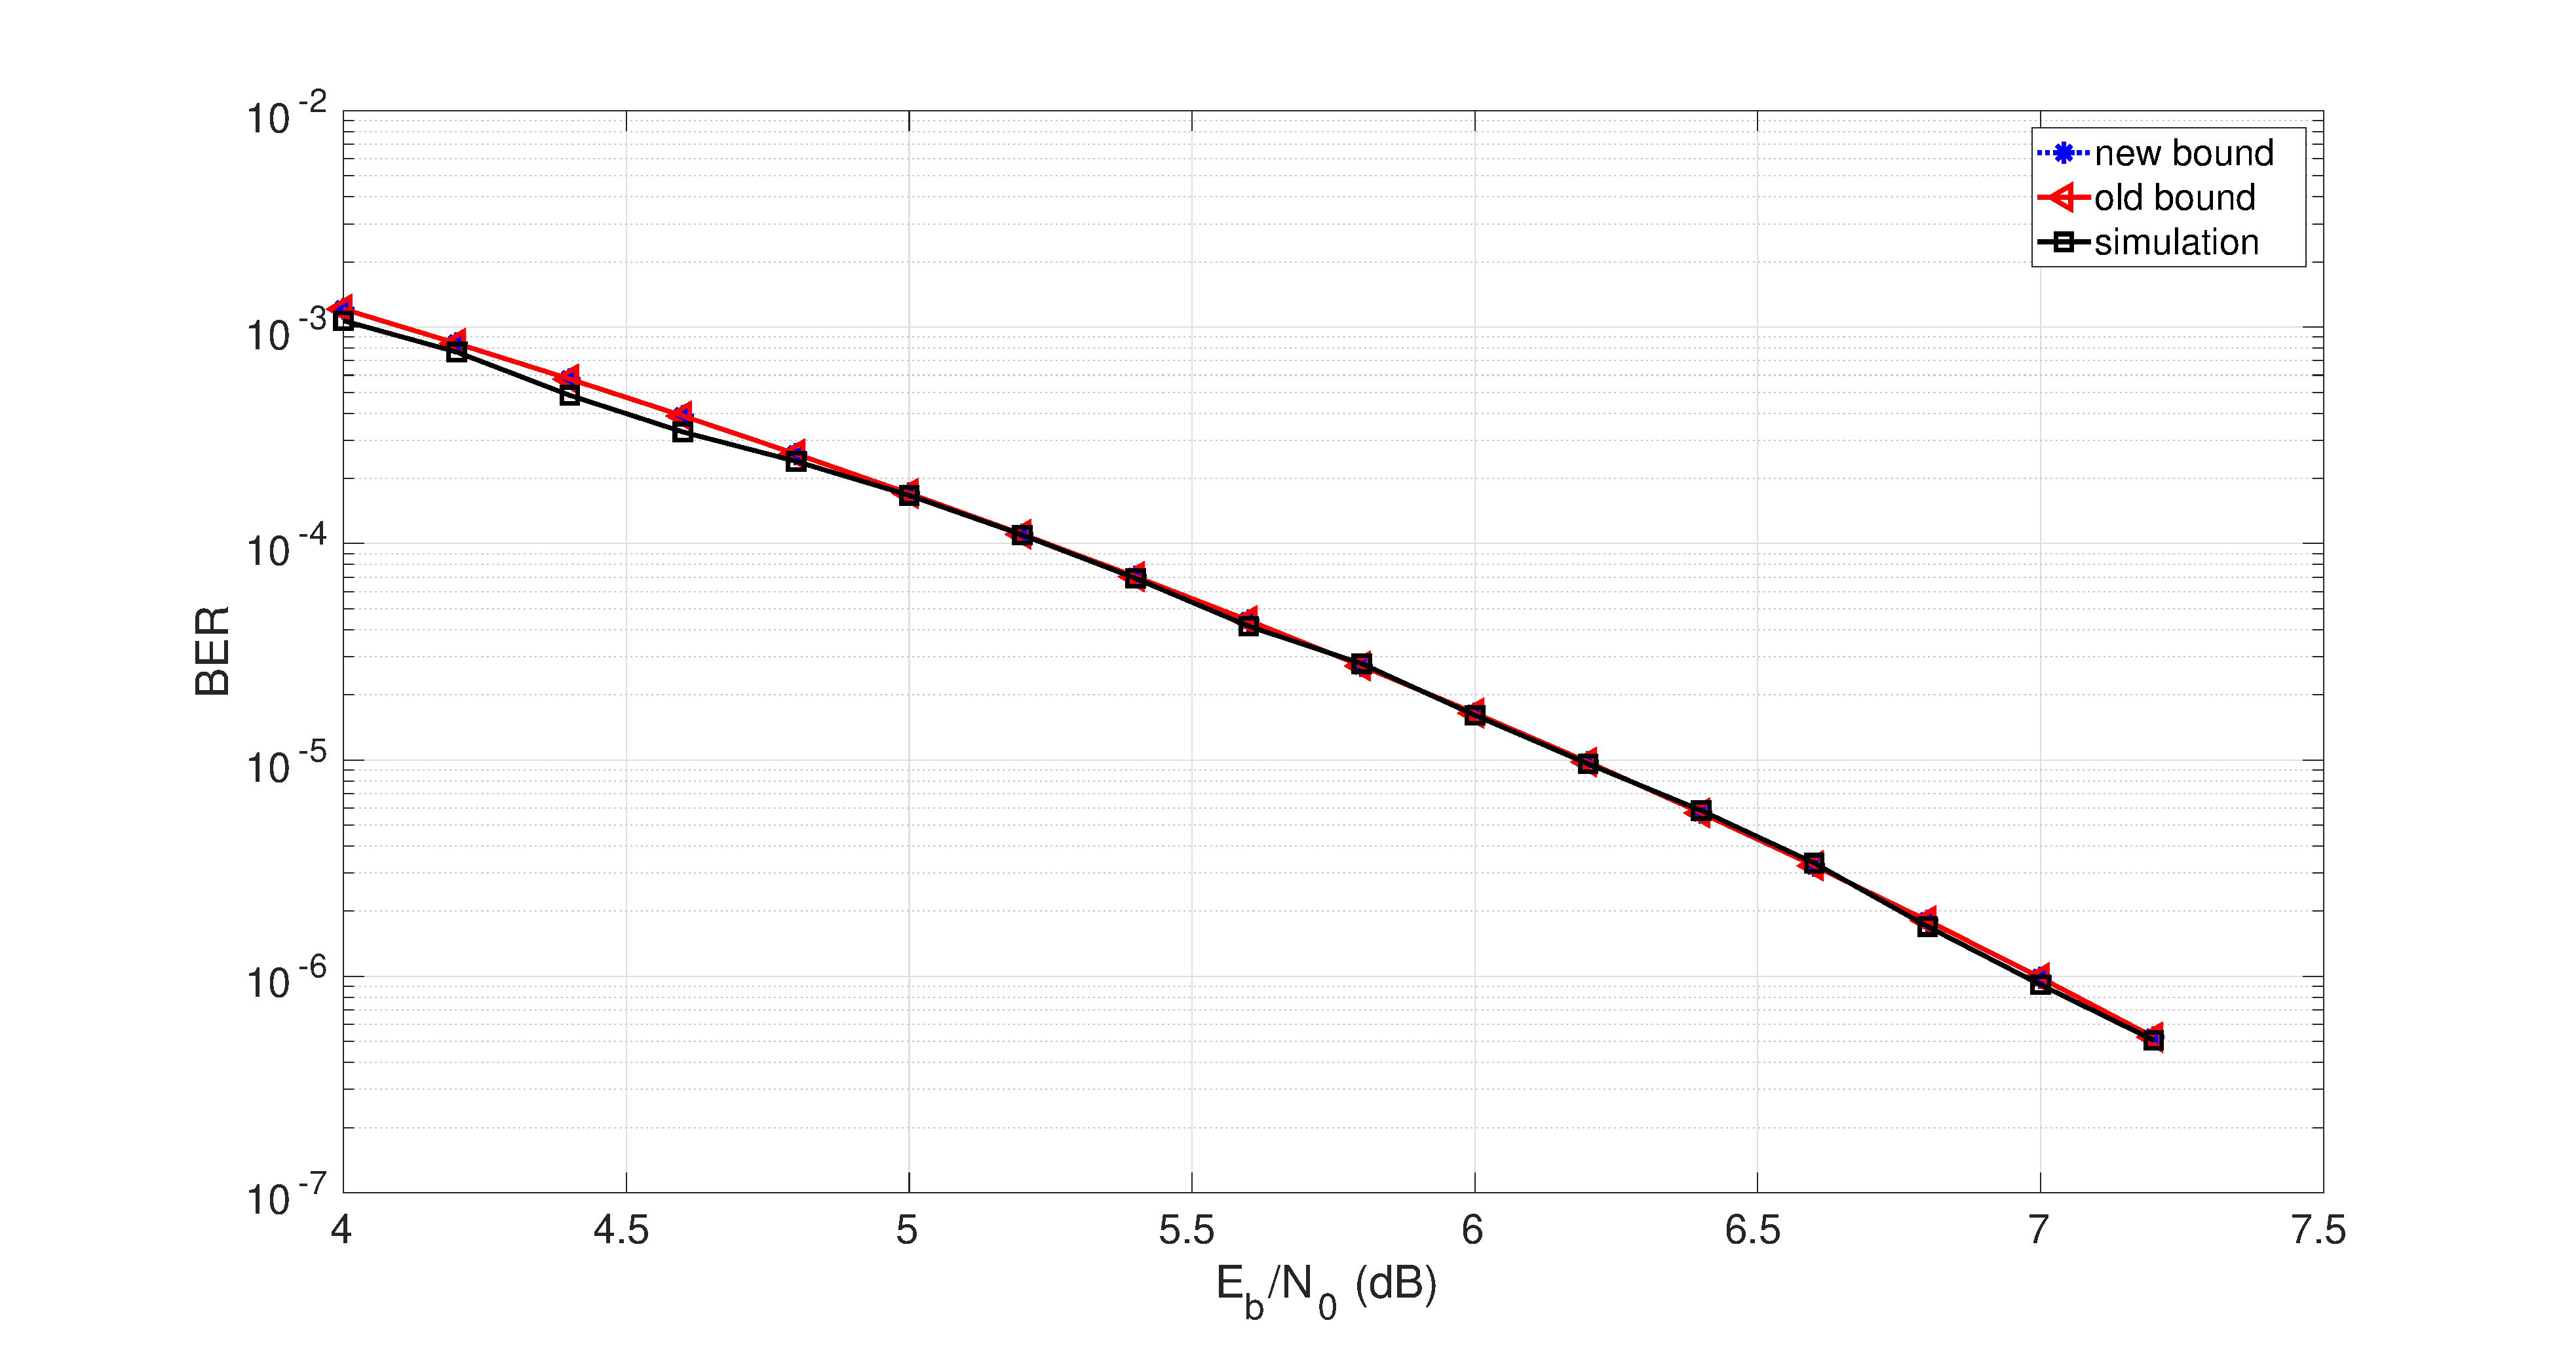
\includegraphics[width=0.8\textwidth]{./Images/RSC_5_7_higher_weights.eps}
%		\caption{Old Bound vs New Bound vs Simulation for 5/7 RSC Code, with higher weights }
%		\label{simFig4}
%		\end{figure}


%		\begin{figure}[h!]
%\centering
%	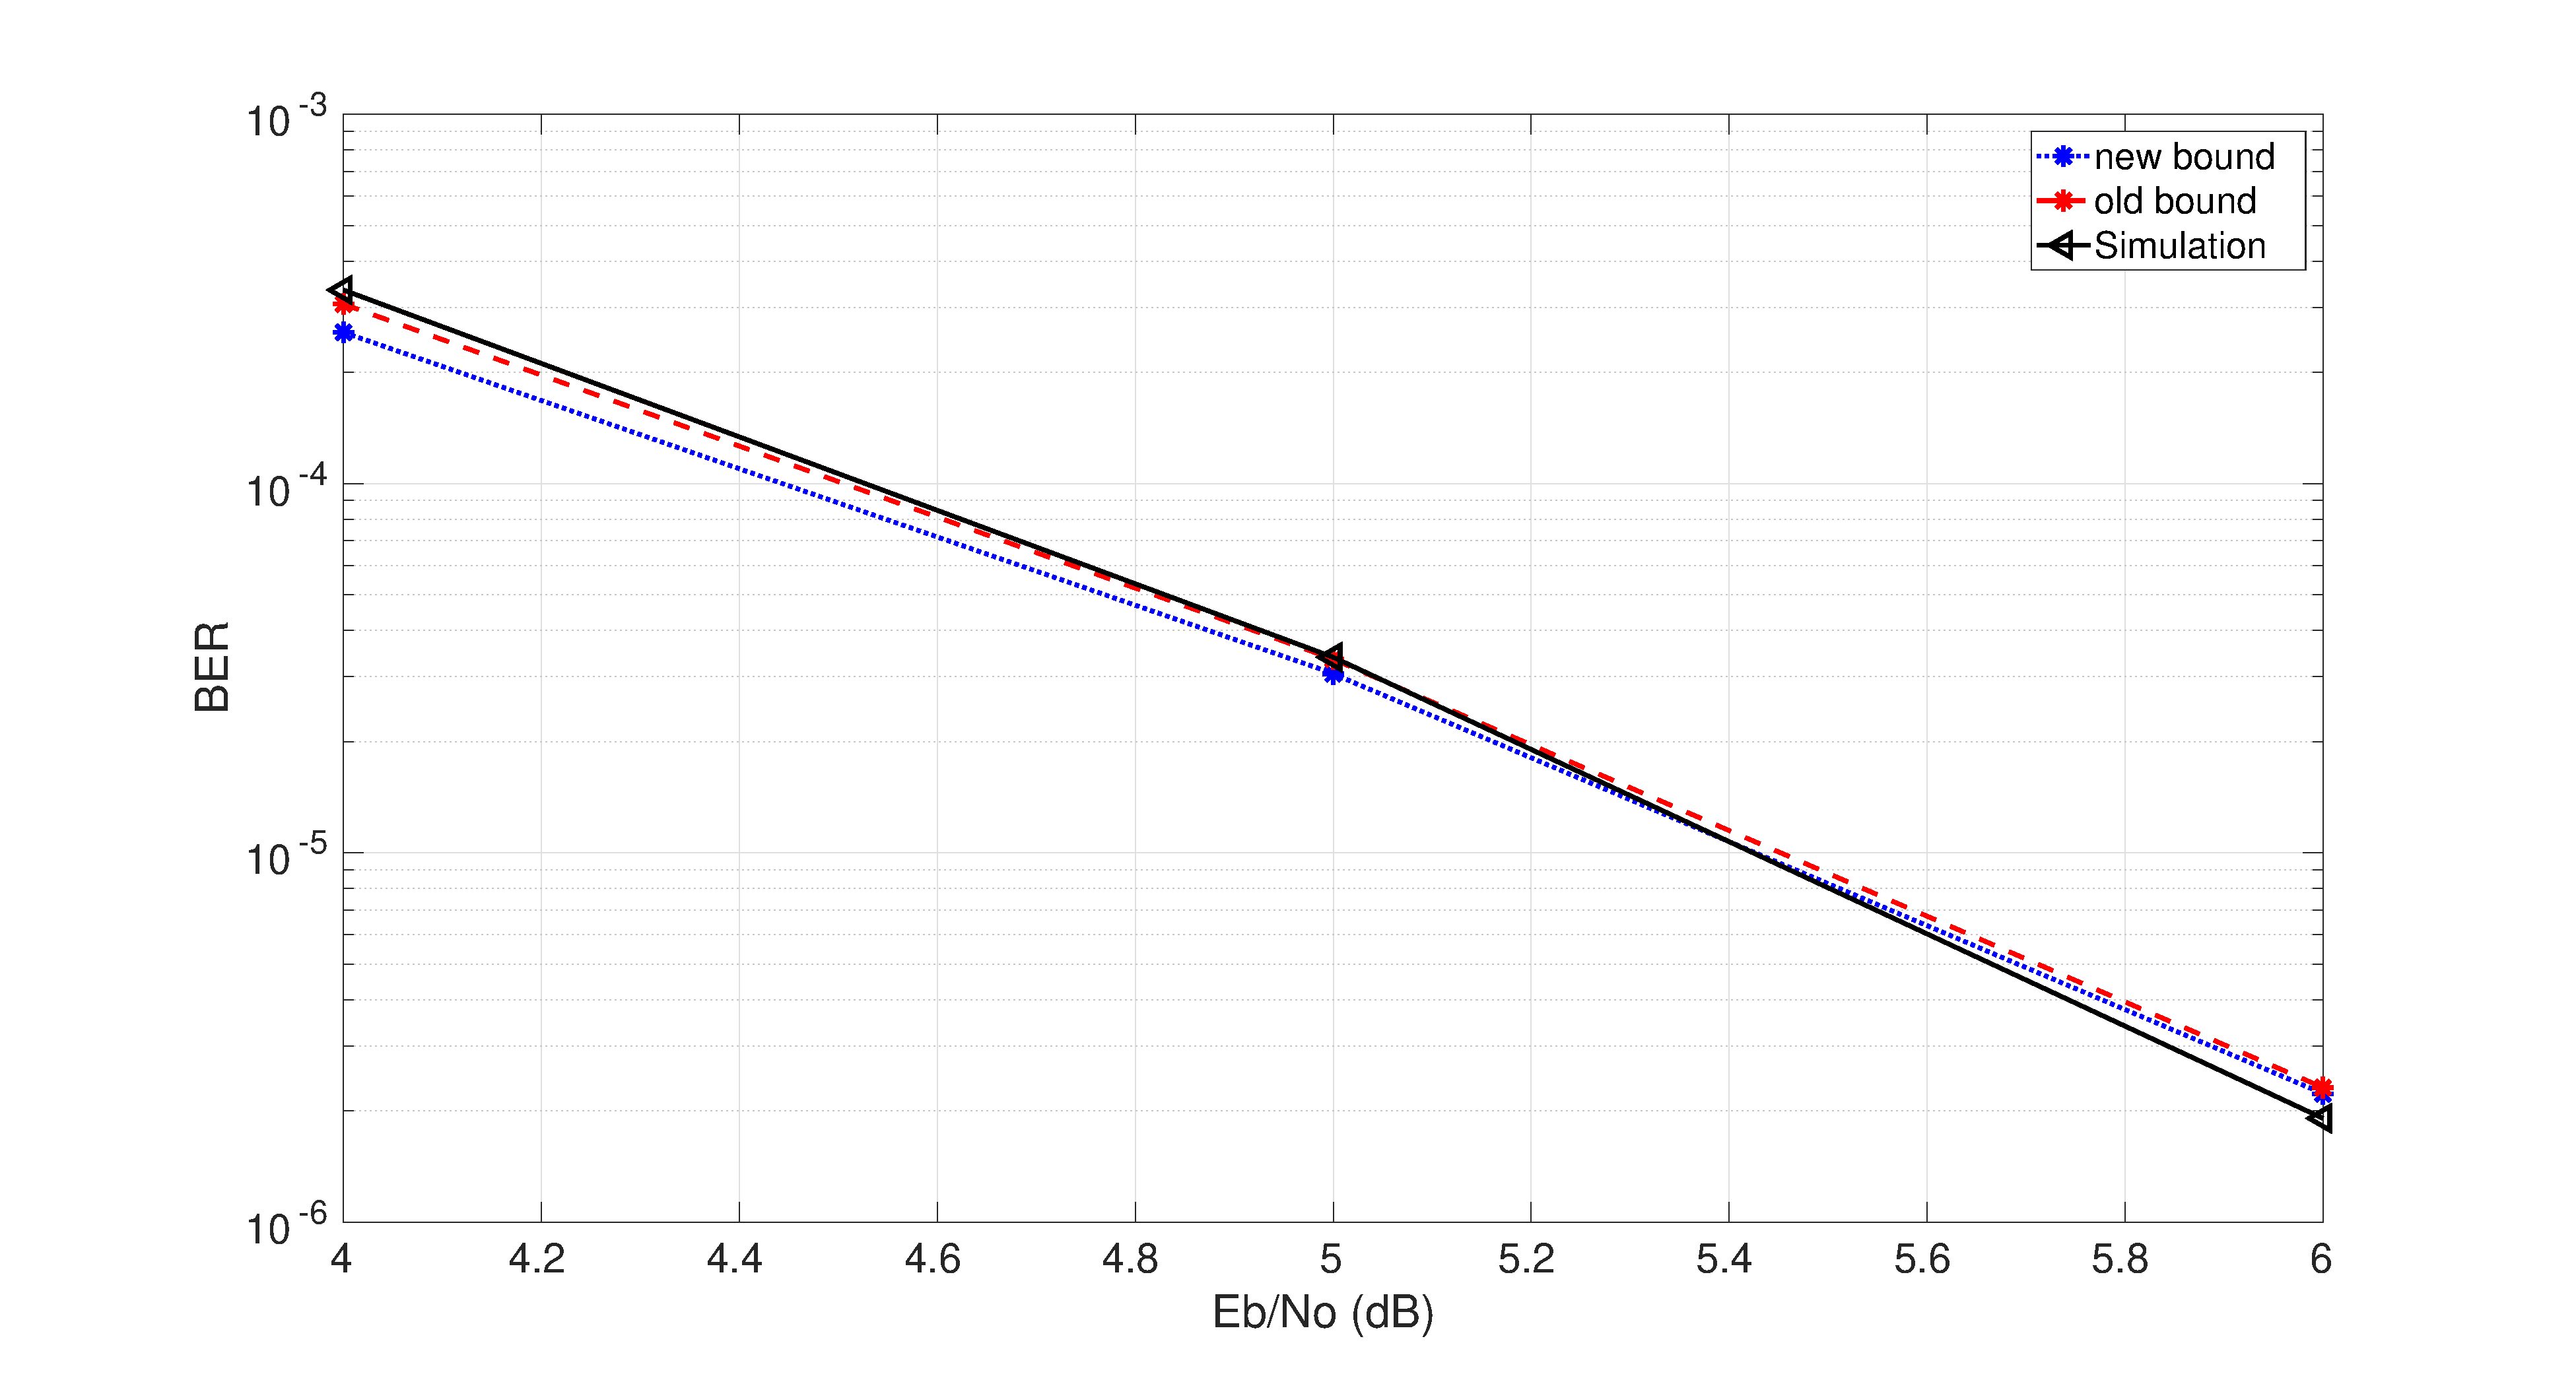
\includegraphics[width=0.5\textwidth]{./Images/RSC_37_21_v2.eps}
%\caption{Old Bound vs New Bound vs Simulation for 37/21 RSC Code, with higher weights}
%\label{simFig5}
%\end{figure}


